\documentclass[sigconf,nonacm]{acmart}
\usepackage{amsmath,tikz}
\graphicspath{{figures/}}
\usepackage{placeins}
\settopmatter{printacmref=false,printfolios=true}
\setcopyright{none}
\acmConference{}{}{}
\acmYear{2026}
\definecolor{ink}{HTML}{17364A}
\title{AirBorder: Coordinating Airport Decisions Across a Passenger Journey}
\settopmatter{authorsperrow=3}
\author{Aravinda Venkatesan}
\affiliation{\institution{University of South Florida}\city{Tampa}\state{Florida}\country{USA}}
\author{Mark Anjoul}
\affiliation{\institution{University of South Florida}\city{Tampa}\state{Florida}\country{USA}}
\author{Phuc Truong}
\affiliation{\institution{University of South Florida}\city{Tampa}\state{Florida}\country{USA}}
\renewcommand{\shortauthors}{Venkatesan, Anjoul, and Truong}
\setlength{\emergencystretch}{2em}
\begin{document}
\raggedbottom
\begin{abstract}
Connecting air passengers must combine a gate deadline, walking times, queues, required procedures and the stops they want to make, while flight information changes. AirBorder is a native iPhone app that keeps these in one journey and shows the next feasible action: when to leave a stop, how long the walk to the gate takes and what changed. Two traveler interviews shaped its requirements, and a high-fidelity Figma prototype was revised after class critiques. The implemented app covers a Tokyo Haneda connection with a gate change, a queue update that proposes a shorter stop, map and camera route guidance, ticket import and walking estimates refined by Apple Health. We plan a within-subjects study that compares AirBorder with Flighty's Connection Assistant on next-action accuracy and deadline interpretation after a gate change.
\end{abstract}
\ccsdesc[500]{Human-centered computing~Human computer interaction (HCI)}
\ccsdesc[300]{Human-centered computing~Ubiquitous and mobile computing systems and tools}
\ccsdesc[300]{Human-centered computing~Empirical studies in HCI}
\keywords{airport connections, passenger decision support, mobile interfaces, explanation, evaluation plan}
\maketitle
\section{Introduction}
\subsection{Problem}
Passengers in an unfamiliar airport must combine boarding deadlines, walking and transport times, queues, baggage and border procedures, and the stops they want to make. A departure time is not a gate-arrival deadline, and a walking estimate may leave out a queue. The information sits in separate places: the ticket, the departure board, airline messages and signs. Our interaction problem is turning these scattered constraints into a feasible next action, and helping the traveler see how that action changes when the information does.

Disruption makes this coordination matter. Our two interviewed travelers described lost rest, missed commitments and extra costs after delays \cite{ref13}. A late inbound flight shortens the usable connection time, and a gate change can lengthen the walk while a traveler is still at a café or lounge. Figure~\ref{fig:motivation} shows the resulting planning task.

\begin{center}
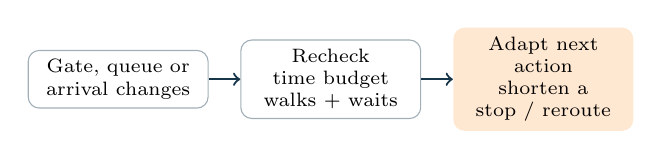
\begin{tikzpicture}[font=\scriptsize]
\node[draw=ink!40,rounded corners,align=center,text width=2.05cm,minimum height=.72cm] (a) at (-.7,0) {Gate, queue or\\arrival changes};
\node[draw=ink!40,rounded corners,align=center,text width=2.05cm,minimum height=.72cm] (b) at (2,0) {Recheck time budget\\walks + waits};
\node[fill=orange!18,rounded corners,align=center,text width=2.05cm,minimum height=.72cm] (c) at (4.7,0) {Adapt next action\\shorten a stop / reroute};
\draw[->,thick,ink] (a)--(b);\draw[->,thick,ink] (b)--(c);
\end{tikzpicture}
\captionof{figure}{Passenger decision after a change: update the time budget while keeping the gate deadline, then adapt the next action.}\label{fig:motivation}
\end{center}

\subsection{End users and approach}
AirBorder is for adults making an airport connection, especially in an airport they do not know well, who want to use the time between flights without risking the next one. It keeps the selected stops, the walk to the gate and the gate-closing time in one journey. It shows when to leave each stop and when the traveler will reach the gate, and it alerts the traveler when the gate or a queue changes. A queue update can lead to a proposed change, such as a shorter lounge visit, that applies only after the traveler accepts it. In aviation, AI support that helped pilots gather information throughout a diversion decision, rather than only recommending an outcome, supported forward reasoning, and decisions were faster when it was combined with a recommendation \cite{ref221}. AirBorder applies this idea to passengers: the time budget and its parts stay visible beside the next action.

\subsection{Scope}
We ask whether travelers can identify the limiting constraint, tell the gate deadline apart from the departure time and revise a plan after a change. The implemented app covers one connection at Tokyo Haneda (HND) Terminal 3, from Bangkok to Los Angeles, plus a variant with a transfer to Narita (NRT). Live flight data, other airports and physical-device testing are outside the current implementation (Section~\ref{sec:status}).

\section{Interview End Users}
We analyzed the recorded answers of two adult travelers, R1 and R2, received on September 28 and 29 \cite{ref13}. Both completed the questionnaire online and independently; it combined categorical items, written accounts and interactive interface tasks, and it showed follow-up questions only when an earlier answer made them relevant \cite{ref2}. We coded the written accounts by situation, need, workaround and consequence, and left contradictions unresolved. Core answers selected later sections through fixed rules, so a reported connection, rest need or difficulty opened only the questions that applied. Each response was stored with the questionnaire version, which let us tell an unanswered item from a question that was never shown; a question not shown is not treated as a negative answer. The interface tasks presented a gate change, a map view and an update that stopped, and recorded the participant's first action, an ease rating and an optional comment. Appendix~\ref{app:interviews} gives both accounts.

\begin{center}\small
\begin{tabular}{@{}p{.27\columnwidth}p{.30\columnwidth}p{.30\columnwidth}@{}}\toprule
Profile & R1 & R2\\\midrule
Age range & 18--24 & 18--24\\
Occupation/field & Student; CS & Student; CS\\
Journeys in 2 years & 3--5 & 3--5\\
Phone; language & iPhone; English & iPhone; English\\
AI tools used & ChatGPT; Claude & ChatGPT; Gemini\\\bottomrule
\end{tabular}
\captionof{table}{Reported participant characteristics.}\label{tab:participants}
\end{center}

Both travelers prioritized leave-by time, routes and an explanation of ``what changed and when.'' R1 also wanted to compare activities; R2 wanted document and transit-entry checks. R1 prefers map-first guidance; R2 prefers camera guidance with the map available. In the interface tasks, neither used the dedicated map-expansion control, and after a gate change R2 wrote ``miss the map directing to new gate.'' R1 reported lost activity time after delays; R2 reported work and rest needs, extra costs and outdated chatbot advice. Both favor free or included facilities. Table~\ref{tab:needs} links these findings to the design.

Their accounts also set the scale of the problem. R1's latest connection, within the past six months, was scheduled for one to under two hours and left no time for the meal and rest R1 wanted, because the inbound flight was late or the onward flight left earlier than expected. Both prefer a scheduled layover of two to under four hours with flexible activities. R2 reported four or more delays in two years, one of four to under eight hours, with rebooking, communication and meal costs and support requests that were only partly met; R2 asked for earlier notice, realistic ranges for how long things take, the effect on the connection and clear support contacts. R2 rated a journey tracker moderately useful, mainly for the current and next step, queue time and required documents. These answers shaped the Flight tab's single timeline, the airline contact on the late-arrival alert and the journey steps.

The interface tasks also showed that ease ratings and behavior can disagree. R1 rated the gate and map tasks very easy, yet chose the camera rather than the map-expansion control; R2 rated the gate task neither easy nor difficult without finding the action. We therefore score what participants do and state in the planned study separately from how easy they say a task was.

The two records share a narrow student, computer-science, English-language and iPhone profile, and R2 gave conflicting flight-frequency answers. The findings motivate requirements and hypotheses; they are not prevalence estimates or usability scores.

\begin{table*}[t]
\begin{minipage}{\textwidth}\centering\small
\begin{tabular}{@{}p{.27\linewidth}p{.33\linewidth}p{.32\linewidth}@{}}
\toprule
Interview evidence & Design response in AirBorder & Evaluation question\\\midrule
Both: leave-by time, routes and changes & Flight tab shows time before the gate closes, leave and gate-arrival times; alerts state the old and new gate & Can they identify when to leave and why?\\[3pt]
R1 map-first; R2 camera-first; R2 missed the route to the new gate & Route tab with Map and Camera views sharing one step; Route button on every alert & Can they reach the route to a changed gate?\\[3pt]
R1 lost activity time; R2 work/rest needs & Ordered stops with editable visit times; queue updates propose a shorter later stop & Can they revise a stop and still meet the deadline?\\[3pt]
R2 outdated advice & Alert time stamps; Help states which data are saved sample data; airline contact on alerts & Can they tell what is confirmed and where to check?\\
\bottomrule
\end{tabular}
\caption{Interview evidence translated into AirBorder features and evaluation questions.}\label{tab:needs}
\end{minipage}
\end{table*}

\section{Current Interface/Solutions}
\paragraph{Primary baseline.} Flighty's Connection Assistant addresses connection feasibility directly. It estimates the steps of a connection, such as deplaning, immigration, baggage, security and the walk to the departure gate, and updates the connection status as conditions change. It does not link that status to a traveler's own stops: someone choosing a meal or a lounge visit still has to work out when to leave. AirBorder makes the chosen stop, its leave time and the effect of a change visible together. Flighty is therefore our comparison system (Section~\ref{sec:eval}).

\paragraph{Related solutions.} TripIt Pro lists airport amenities with walking directions, and airline apps such as Fly Delta send gate notifications and offer rebooking. Both interviewees use Google Flights, airline or airport apps and ChatGPT, and R2 reported effort moving chatbot advice into an itinerary \cite{ref13}. Signs, departure boards and staff remain the main alternatives in the airport.

\paragraph{Related research.} Explaining why a system behaved as it did improved understanding and trust, whereas why-not explanations lowered understanding \cite{ref7}. AirBorder therefore leads with why the plan changed and keeps blocked alternatives secondary. Showing sources reduced reliance on incorrect answers from a language model, while explanations alone increased reliance on correct and incorrect answers alike \cite{ref219}; explanations reduced overreliance when they made an answer cheaper to verify \cite{ref220}. AirBorder therefore shows the values behind a proposal, such as the extra queue minutes and the new visit length, so a traveler can check them. In a controlled transit experiment, quantile dotplots and CDFs led to better leave-time decisions than a single predicted time or text uncertainty \cite{ref8}. The level at which uncertainty is shown also matters: uncertainty attached to individual reasoning steps reduced users' independent verification of a language model's answer \cite{ref222}. AirBorder currently shows single average estimates; a range for the leave-by result is planned, with the airline kept visible as the place to confirm the gate.

\section{Initial Design}\label{sec:initial-design}
\subsection{High-fidelity prototype}
Our high-fidelity prototype is an interactive Figma design for iPhone 13 (390 $\times$ 844 points) with four tabs: Flight, Layover, Route and Profile. It uses a navy ticket card, yellow gate signs and the Outfit typeface, and real Haneda Terminal 3 photographs. Its scenario is a Bangkok--Haneda--Los Angeles trip: the traveler lands at 11:15, and the onward flight NH~106 departs at 18:00 from Gate~105, which closes at 17:25. The Flight tab shows the ticket and ``Your plan''; Layover lists airside venues, landside places and city options; Route gives step-by-step directions to the gate; Profile holds walking data, connected accounts and settings. Prototype links simulate a gate change to 108A, a longer café queue, ``return now'' and ``boarding at risk'' alerts, and a transfer to Narita.

\subsection{Screens and flows}
\emph{Onboarding.} A welcome screen and three short pages explain the layover timeline (departure, layover, destination), the time before the gate closes and a route walked at the traveler's own pace; Skip is available on each page.

\emph{Flight.} The navy ticket shows the route, the departure time and a yellow gate sign; below it, ``Your plan'' states the time before the gate closes and a Route button. Each selected stop has a card with a timeline from now to leave, at the gate and gate closing. Journey details list both flights, baggage, the return flight and a Call ANA action; Journey steps show the checkpoints from arrival to boarding. When a timing situation holds, the plan is replaced by a countdown and a Route button in the matching color: amber for return now and red for boarding at risk.

\emph{Layover.} Three segments separate Airside venues near the gate (filtered by Rest or Food \& drink), Landside places such as a private workspace booth, an electronics shop with its phone number and the Terminal~3 and Terminal~2 observation decks, and City \& transfer options such as the Haneda Innovation City sky deck and the Keikyu line. Each airside card shows the walk from the traveler and back to the gate and an Add button; landside and city cards show the time to return through security.

\emph{Route.} A title names the destination gate, a Map/Camera switch sits above a walking-time strip, and a numbered step card carries the written instruction with Previous, Next step and End. Route options open below the card.

\emph{Profile.} Saved flights, Connected accounts (Apple Health, Gmail, Calendar), Previous trips, Step-free routes, Language, Privacy, Help \& information, About, Replay tutorial and Reset preferences, which returns stops, journey steps and route settings to their starting state.

\subsection{Changes after the class critiques}
The instructor and classmates reviewed the prototype; we received 14 substantive classmate responses. Their points, and what we changed, were:
\begin{itemize}
\item \textbf{Gate changes must be prominent} (instructor). A gate update now opens an Alerts screen automatically, showing ``Gate 105 $\rightarrow$ 108A'', the closing time and the walk. The full identifier 108A replaces 105 on the ticket, the plan and the route.
\item \textbf{One working Back control} (instructor; peers). Each screen has one back icon. The camera view has an Exit camera button, and the last route step has an End button.
\item \textbf{Onboarding} (instructor). The welcome and three onboarding screens run once, with Skip; Profile offers Replay tutorial.
\item \textbf{Clear plan building} (four peers). ``Add caf\'e'' changes to an added state, stops appear in order with visit times, and they can be edited, removed and reordered in My plan.
\item \textbf{Integrated directions} (four peers). Map and Camera views share the same route step and written instruction, so switching views keeps progress. Route options offer Direct, Step-free and Less crowded walks.
\item \textbf{Lounges, tickets, transfers and walking} (several peers). We added a lounge detail page with a floor map, ticket import by camera and PDF, a step-by-step Haneda--Narita transfer, and walking estimates that start from average times and use the traveler's own pace when Apple Health is connected.
\item \textbf{Queue and crowd changes} (three peers). A queue update recalculates the plan and, if the traveler would reach the gate late, proposes shortening a later stop, with Apply, Keep my plan and Undo.
\end{itemize}
Classmates also praised the colors, the introductory guidance, the facility cards and the airside/landside grouping, so we kept them unchanged. Figure~\ref{fig:screens} shows the revised screens as implemented.

Several suggestions were changed rather than adopted literally. The critique asked us to weigh a dedicated plan tab against prominent entry points; we kept the four original tabs and made the plan reachable from the Flight tab (``My plan'') and from each venue card, because the plan is meaningful only next to the gate and its closing time. Our earlier design asked travelers to set a walking pace; in response to the walking-estimate critique, it became an automatic estimate that uses the traveler's own airport walks and Health data when available and never asks travelers to judge their own pace. Queue updates do not reorder or remove stops; they propose the smallest change to one selected stop, and the traveler decides. Each of these keeps the traveler in control of the plan while still answering the critique.

\begin{figure*}[t]
\centering
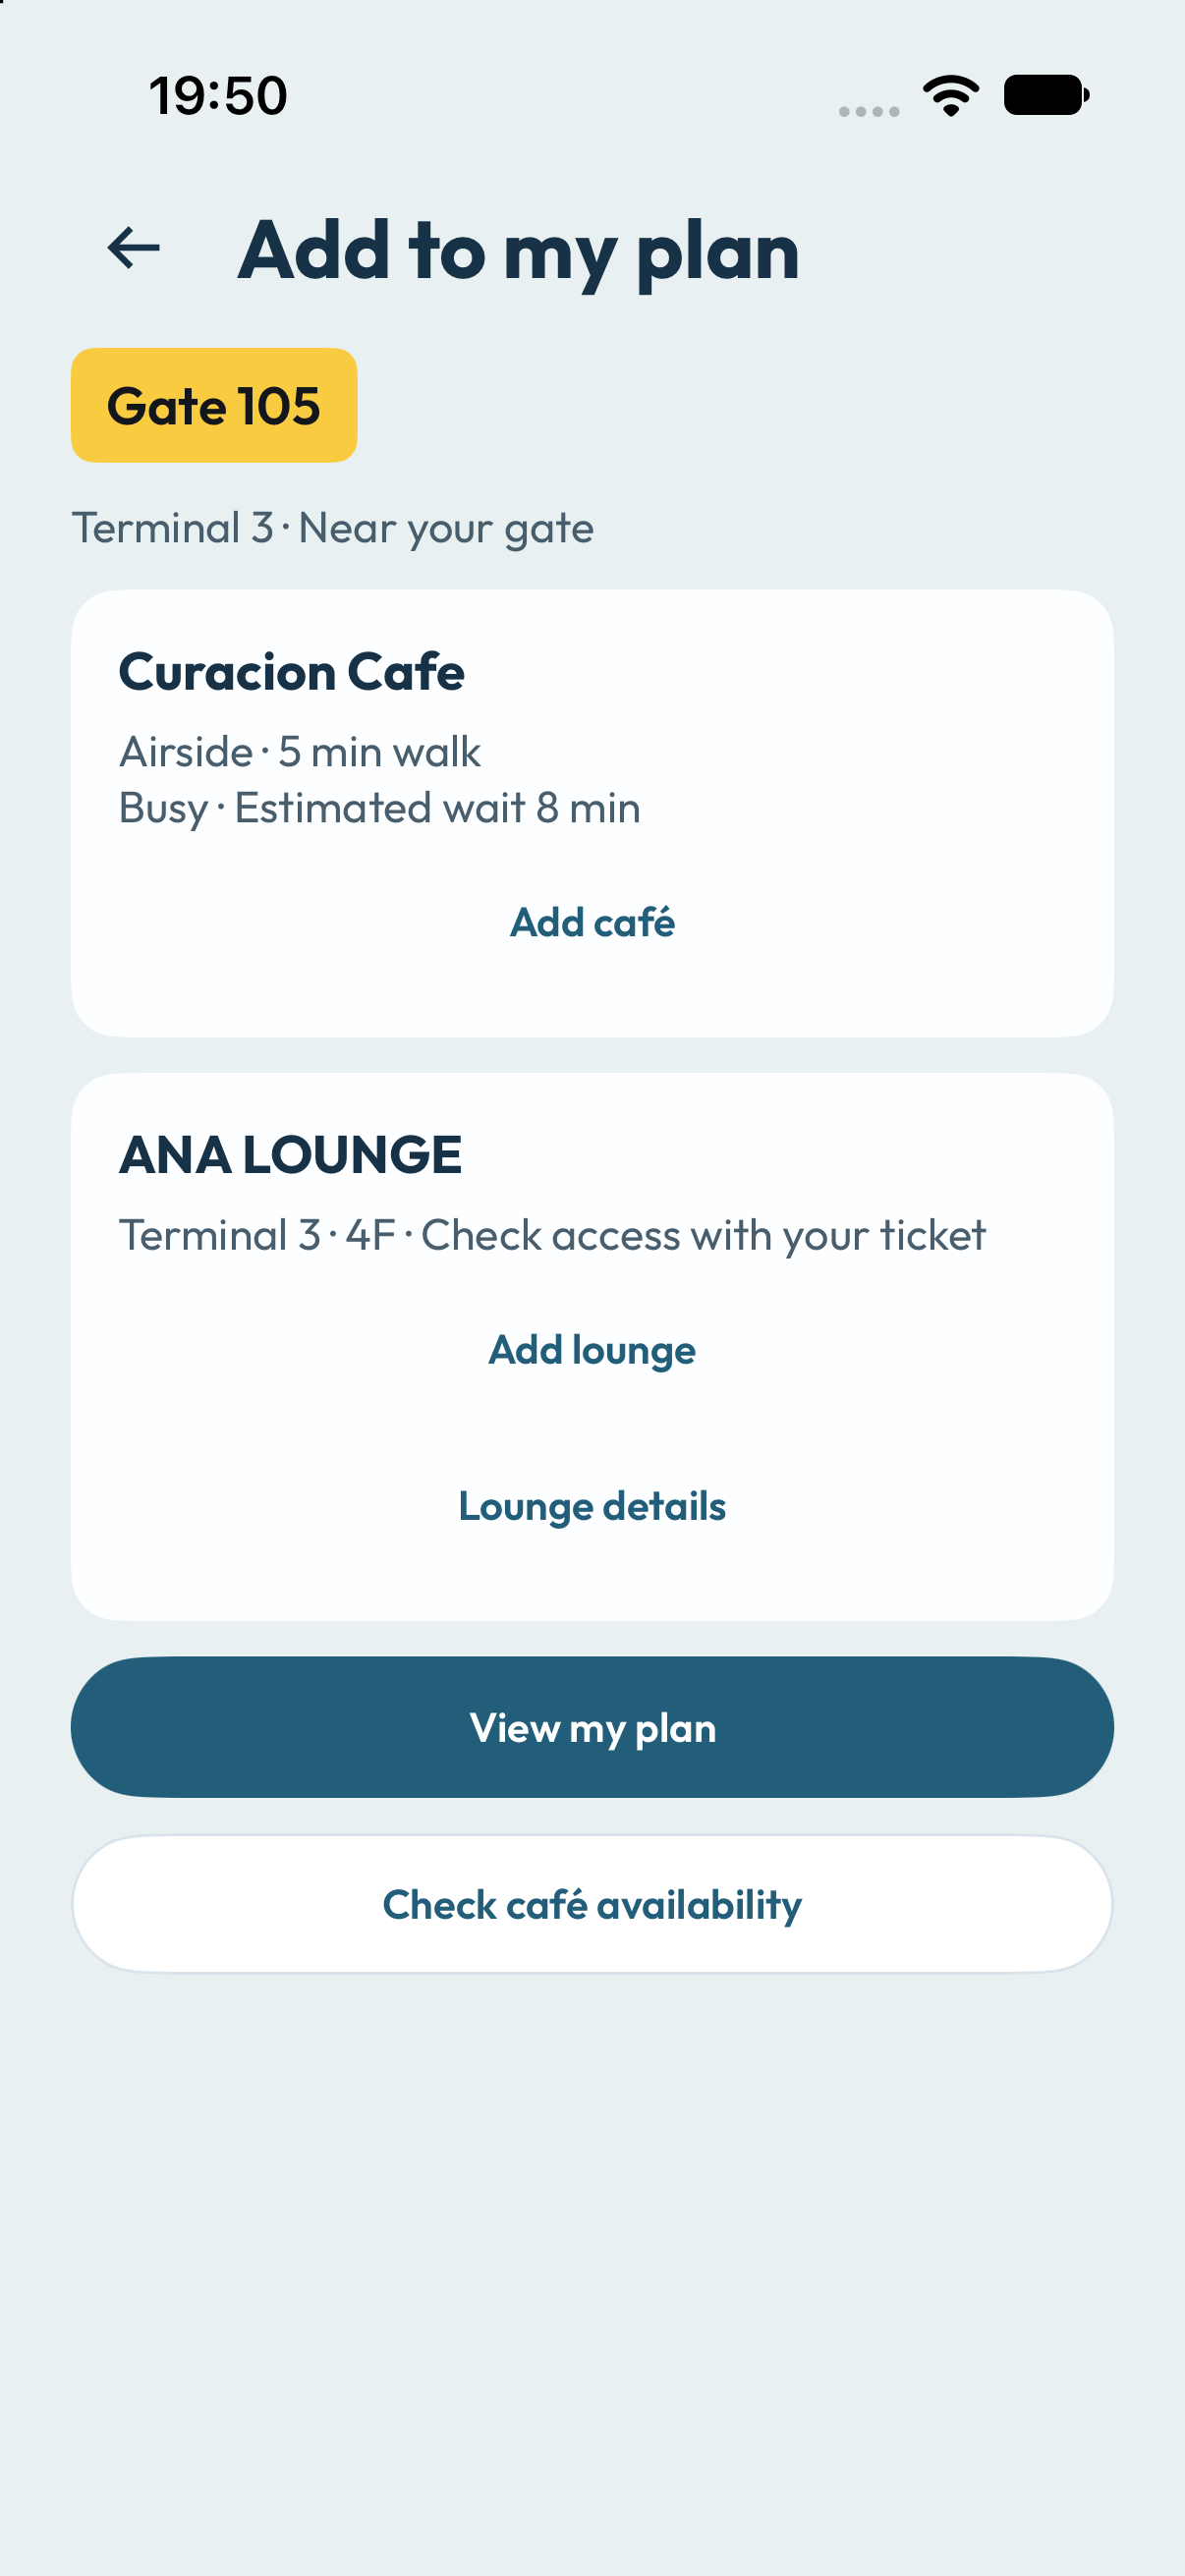
\includegraphics[width=.2\textwidth]{App-AddToPlan.png}\hfill
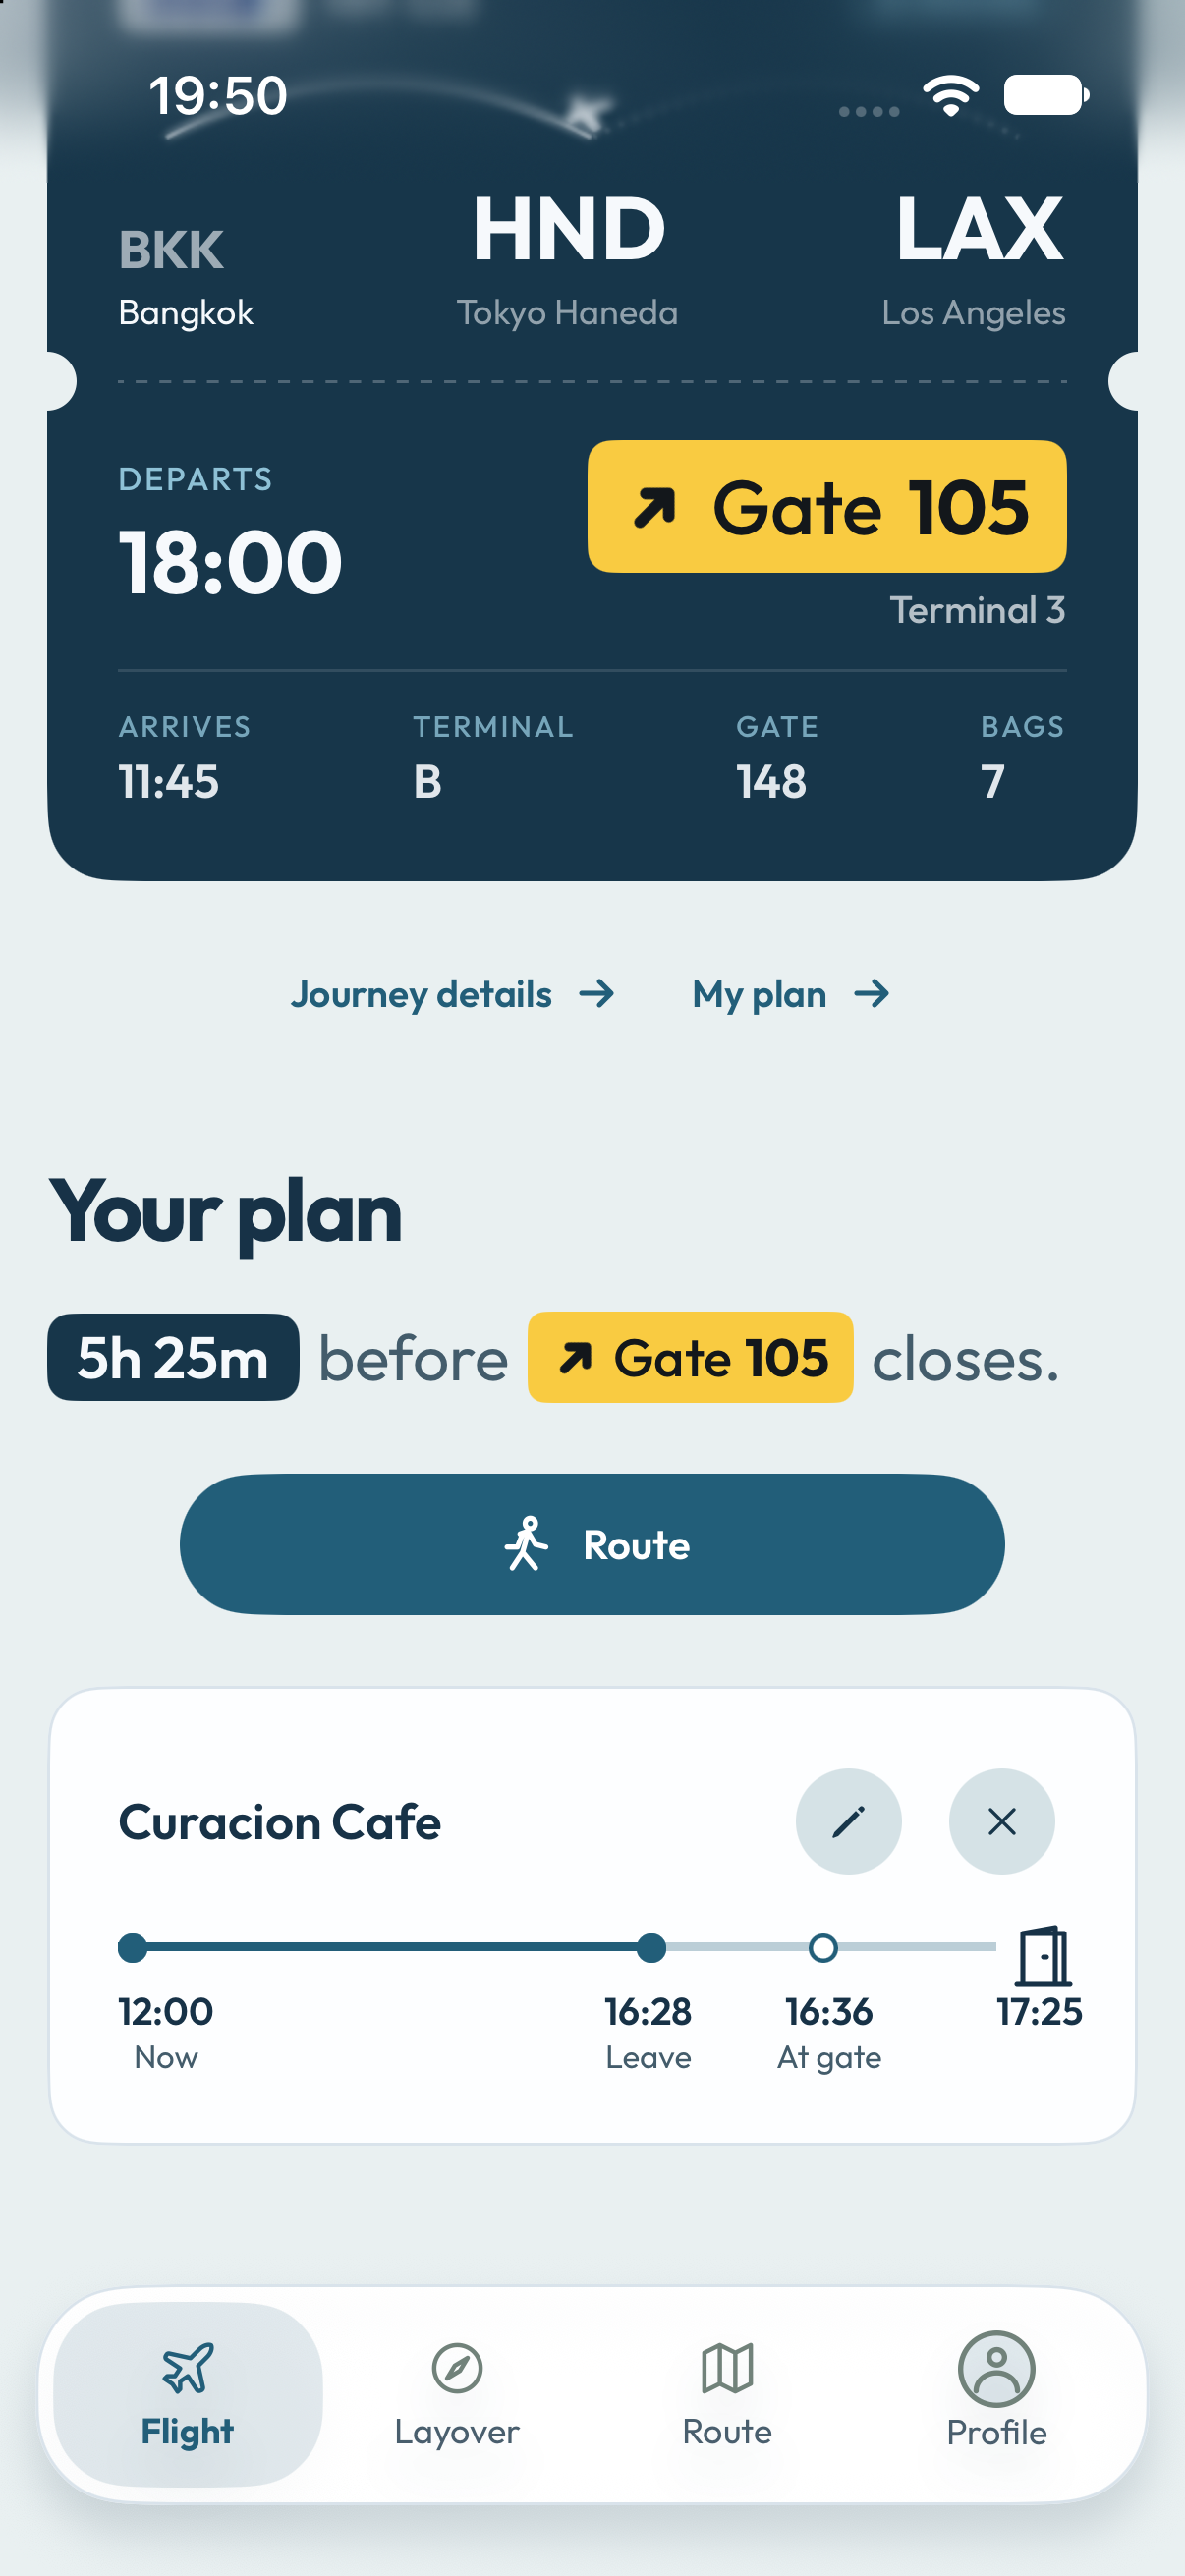
\includegraphics[width=.2\textwidth]{App-Flight.png}\hfill
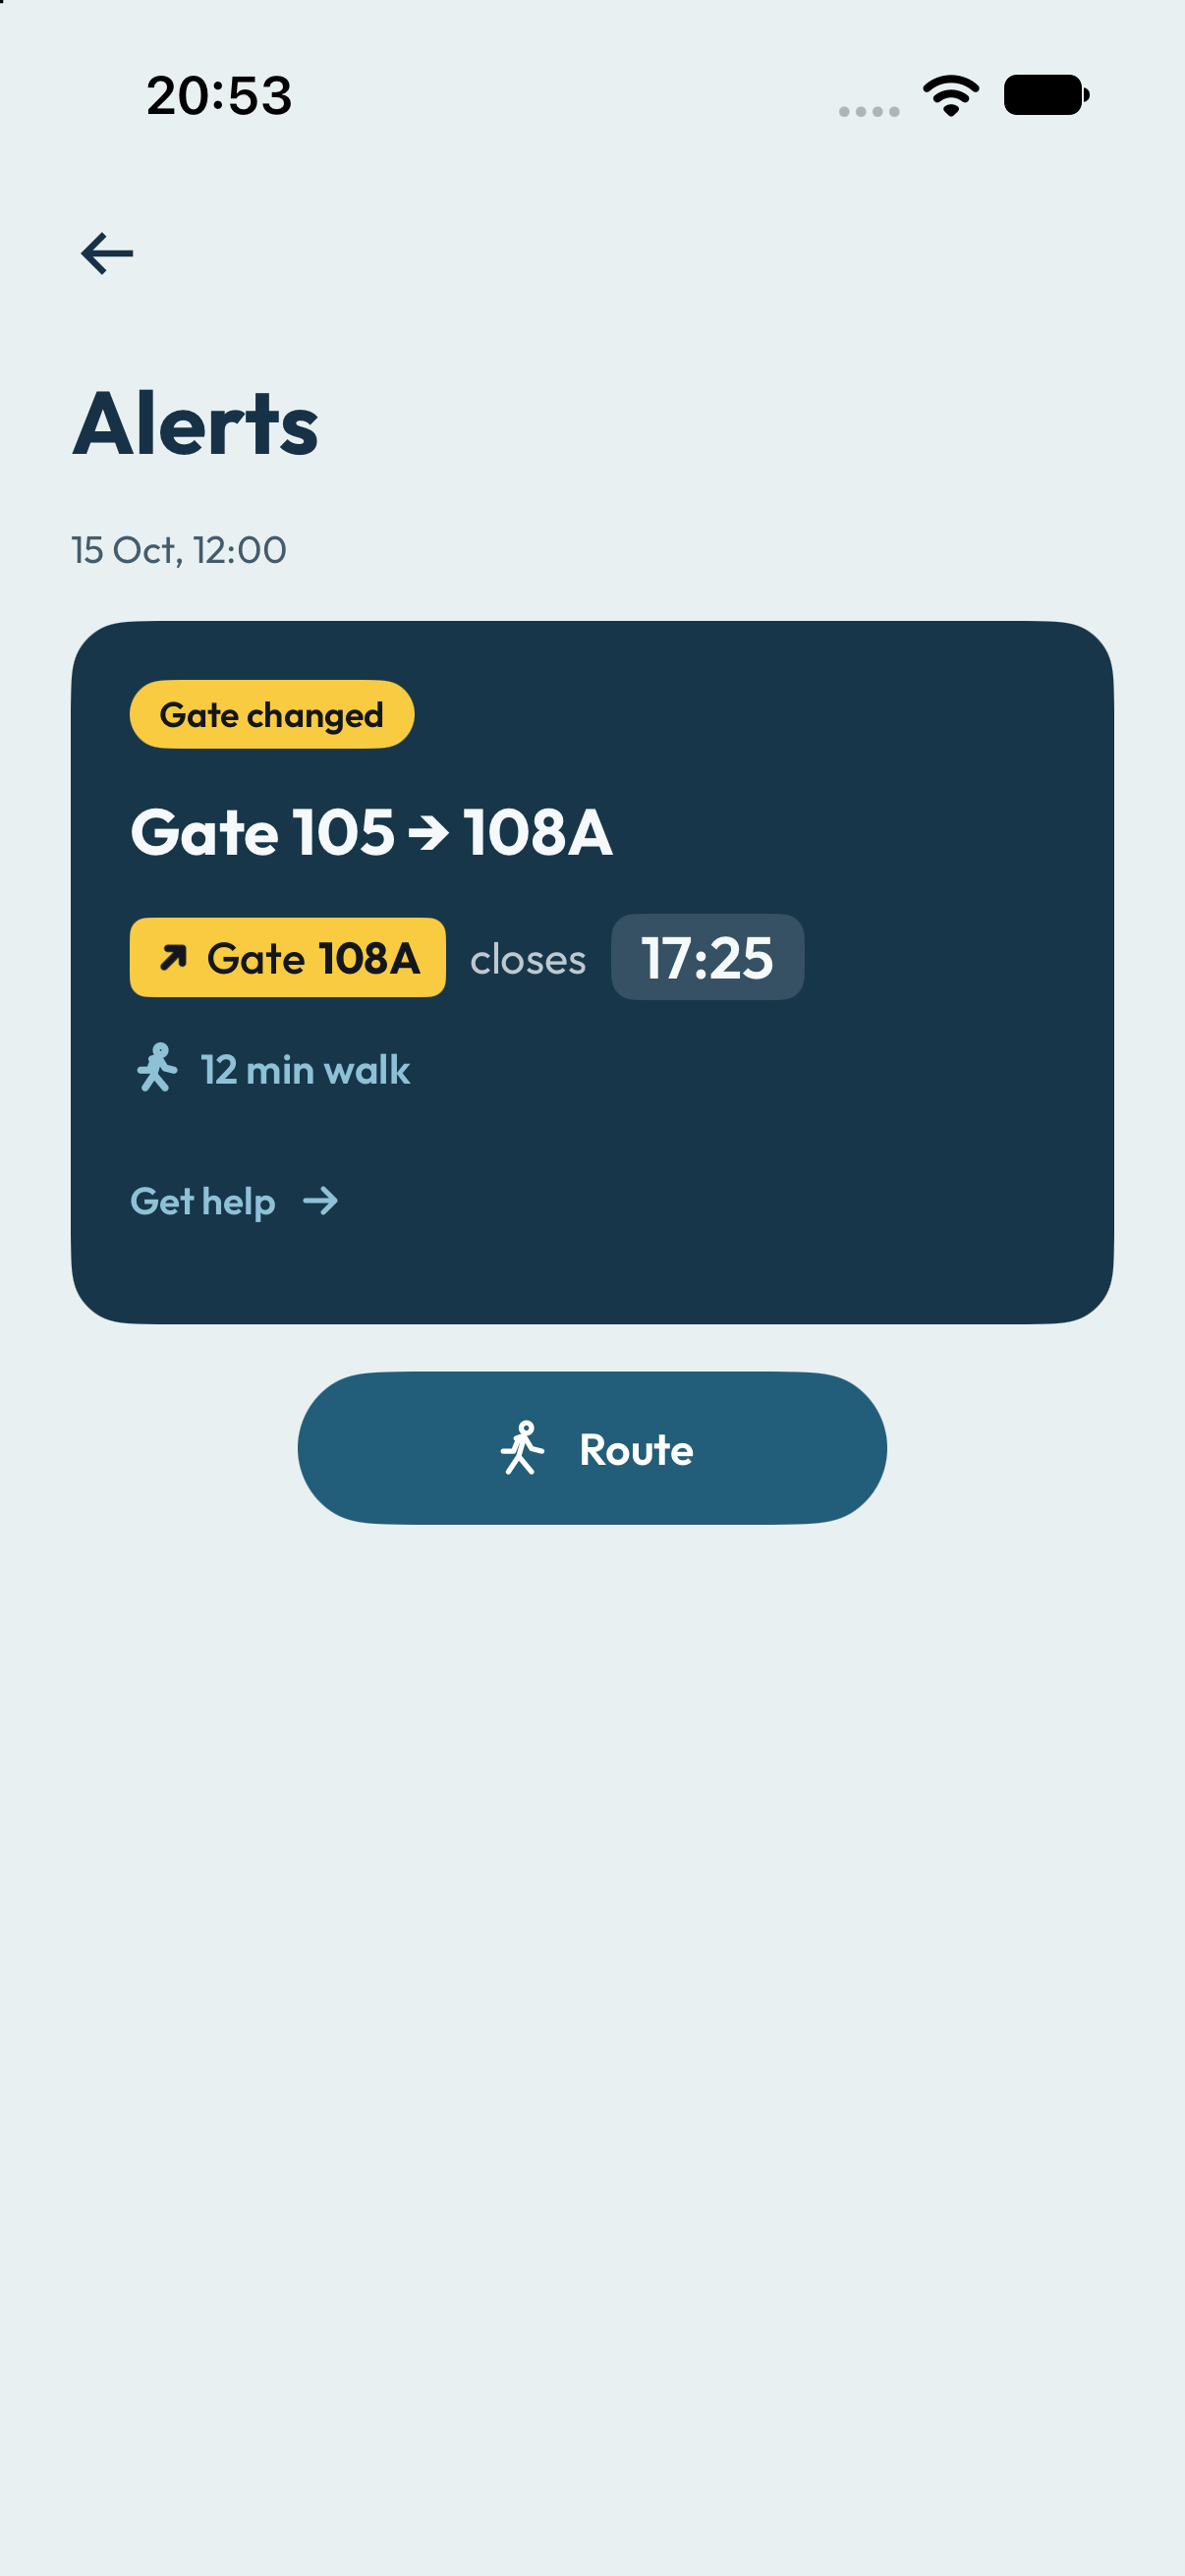
\includegraphics[width=.2\textwidth]{App-GateAlert.png}\hfill
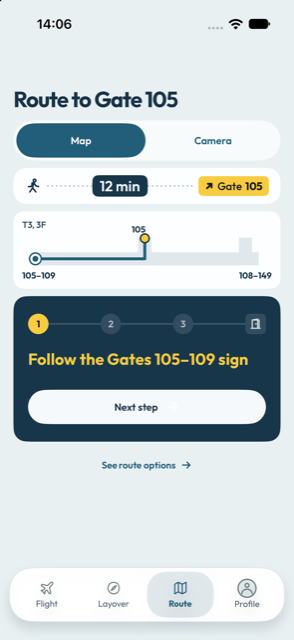
\includegraphics[width=.2\textwidth]{App-Route.png}
\caption{The implemented app on an iPhone simulator. From left: adding a café or lounge near the gate; the Flight tab with the plan timeline (now, leave, at gate, gate closes); the gate-change alert, with the full identifier 108A and a Route action; and the Route tab, whose Map and Camera views share the current step.}\label{fig:screens}
\Description{Four phone screens: an Add to my plan list with Curacion Cafe and ANA LOUNGE; the Flight tab with a navy ticket, Gate 105 and a timeline from 12:00 to 17:25; an Alerts screen showing Gate 105 to 108A, closing at 17:25 with a 12-minute walk; and a Route to Gate 105 screen with Map selected and the step "Follow the Gates 105--109 sign".}
\end{figure*}

\section{System}
Functionally, AirBorder lets the traveler see their connecting flight and the time left before the gate closes; add caf\'es, lounges and a landside visit to an ordered plan with leave and gate-arrival times; receive alerts when the gate changes or time runs short; accept or decline a proposed change after a queue update; follow step-by-step directions to the gate on a map or with the camera; track required steps such as security and passport control; add a ticket by camera, PDF or manual entry; and refine walking estimates with Apple Health. This section gives the technical details needed to rebuild these features.
\subsection{Platform and architecture}
AirBorder is a native iPhone app written in Swift and SwiftUI for iOS 18 or later. A single observable journey store holds the selected plan, the journey checkpoints, the latest flight report, alert records, the chosen route and walking data; every tab reads it, so a change appears everywhere at once. The store is saved on the device as JSON in user defaults. Vision recognizes text in ticket photos and in signs seen by the camera, PDFKit reads ticket PDFs, AVFoundation provides the camera, and HealthKit supplies walking speed. All recognition runs on the device.

The code is organized in three layers. \texttt{Model/} holds plain value types and pure functions: the journey and flight legs, the plan engine, the situation rules, the checklist, walking estimates and ticket parsing. They have no user-interface code, so the unit tests call them directly. \texttt{App/} holds the store, the root view and tab navigation. \texttt{Features/} holds one folder per tab (Flight, Layover, Route, Profile) and the onboarding flow; \texttt{Design/} holds the shared colors, the Outfit typeface, cards, buttons and information sheets taken from the Figma components. Each tab has its own navigation stack, and alerts, journey details and import screens are pushed onto the Flight stack, so a single back icon always returns to the screen that opened them.

\begin{figure}[t]
\centering
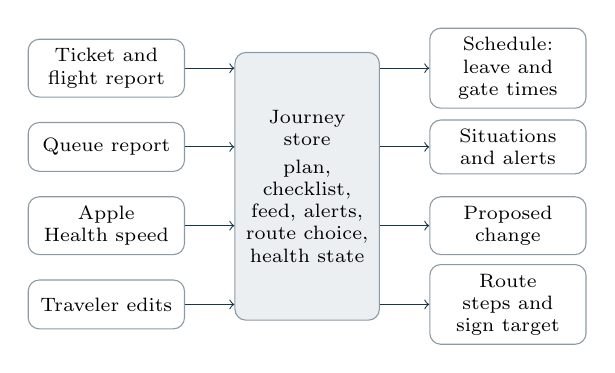
\begin{tikzpicture}[font=\scriptsize,box/.style={draw=ink!50,rounded corners,align=center,text width=1.75cm,minimum height=.62cm}]
\node[box] (in1) at (0,1.5) {Ticket and flight report};
\node[box] (in2) at (0,.5) {Queue report};
\node[box] (in3) at (0,-.5) {Apple Health speed};
\node[box] (in4) at (0,-1.5) {Traveler edits};
\node[box,fill=ink!8,text width=1.6cm,minimum height=3.4cm] (st) at (2.55,0) {Journey store\\[2pt]plan, checklist,\\feed, alerts,\\route choice,\\health state};
\node[box] (d1) at (5.1,1.5) {Schedule: leave and gate times};
\node[box] (d2) at (5.1,.5) {Situations and alerts};
\node[box] (d3) at (5.1,-.5) {Proposed change};
\node[box] (d4) at (5.1,-1.5) {Route steps and sign target};
\foreach \i in {1,2,3,4}{\draw[->,ink] (in\i.east)--(st.west|-in\i.east);\draw[->,ink] (st.east|-d\i.west)--(d\i.west);}
\end{tikzpicture}
\caption{Data flow in the app. Inputs change the journey store; the schedule, situations, proposals and route steps are recomputed from it, and every tab reads the results.}\label{fig:dataflow}
\Description{Four inputs (ticket and flight report, queue report, Apple Health speed, traveler edits) feed a central journey store, which produces four derived outputs: the schedule, situations and alerts, a proposed change, and route steps with the sign target.}
\end{figure}

Figure~\ref{fig:dataflow} shows how state moves through the app. Only inputs are stored: the plan, the checklist, the latest flight report, the alert records, the route preference, the Health connection state, the saved flights and the profile. Everything the traveler sees about timing is derived on demand from those inputs, so there is no second copy that could go stale. The store writes a versioned JSON record (\texttt{journeyState.v1}) to user defaults after every change and reads it at launch; a UI-test launch argument resets it. The walking speed from Health is not stored: it is read again from Health each time.

A separate Cloudflare Worker written in JavaScript holds provider credentials and exposes authenticated endpoints for flight status and search, departure and arrival boards, an airport facility registry, entry requirements, reminders, optional model explanations and revisioned journey storage. The app does not call the Worker yet: it ships one saved sample journey, and Help states that its flight times, gates, venues and queues are not live. The flight report is modeled on the Worker's flight-status response (a gate and a receipt time), so connecting the two replaces the sample report without changing the situation rules.

\subsection{Plan timing}
All times are airport-local minutes. Let $s_0$ be when stops begin (16:00 in the sample), and let each selected stop $i$ have a queue wait $q_i$ and visit length $v_i$. With $w(a,b)$ the walking time between places, the start of stop $i$ is $t_i = e_{i-1} + w(p_{i-1},p_i)$, where $e_{i-1}$ is when the previous stop ends ($e_0=s_0$, $p_0$ the start point), and the stop ends at $e_i = t_i+q_i+v_i$. The traveler leaves the last stop at $e_n$ and reaches the gate at
\[A = e_n + w(p_n,\mathrm{gate}).\]
The airline's gate-arrival target $D$ is 20 minutes before the gate closes (17:05 for a 17:25 close). With no stops, the leave-by time is $D$ minus the walk to the gate.

Table~\ref{tab:worked} works through the sample plan. With a café (8-minute wait, 20-minute visit) and the ANA LOUNGE (28 minutes), the traveler reaches the gate exactly at 17:05. When the café wait rises to 18 minutes, the same computation gives 17:15, ten minutes past the target. Shortening the lounge to 18 minutes restores 17:05; keeping both stops as they are still reaches the gate before it closes, but after the target. The Flight tab shows these times on a timeline from now to the gate closing (Figure~\ref{fig:screens}).

\begin{table}[t]\small\centering
\begin{tabular}{@{}lccc@{}}\toprule
 & Planned & Longer queue & Apply \\\midrule
Café (wait + visit) & 16:00--16:28 & 16:00--16:38 & 16:00--16:38\\
ANA LOUNGE & 16:33--17:01 & 16:43--17:11 & 16:43--17:01\\
At the gate & 17:05 & 17:15 & 17:05\\\bottomrule
\end{tabular}
\caption{Worked timing for the sample plan at average walking pace (5-minute walk from café to lounge, 4 minutes from lounge to gate; target 17:05, gate closes 17:25).}\label{tab:worked}
\end{table}

Walking times come from a table of average minutes between Terminal 3 places at 4.2~km/h. If the traveler connects Apple Health, the app reads walking speed and, together with the speed from recorded airport walks on previous trips (equal weight), rescales each walk: $w' = \lceil 70\,w / (1000\,k/60)\rceil$ for pace $k$ in km/h. Without either source, the average times apply.

The walking estimate follows a consent path. Profile $\rightarrow$ Connected accounts explains what is read before the system permission sheet appears, and the app asks only to read one Health type, walking speed, which iPhone and Apple Watch record. It takes the average of the last 28 days of samples and converts it from metres per second to km/h. Speeds outside 1--9~km/h are ignored. If the traveler declines, the account has no samples, or Health is not available on the device, the estimate falls back to the airport walks and then to average times. Removing Health in Profile sets the connection to removed, clears the speed and recomputes every time at once; the app never labels a pace as slow or fast. The three recorded airport walks in the sample (840~m in 12 minutes, 630~m in 9 and 1{,}050~m in 15) give 4.2~km/h, the same as the average, so the sample journey only changes when Health is connected.

\subsection{Situations and alerts}
The app evaluates five situations from the current inputs, most urgent first. With $c$ the gate-closing time, $n$ the current time and $g$ the walk to the gate, the spare time is $c-(n+g)$. If it is negative, the traveler would arrive after the gate closes, and the app offers boarding assistance with the airline's phone number. If it is under 10 minutes, boarding is at risk. If the traveler is past the leave time with more spare time, the app says to return now. Separately, a gate in the flight report that differs from the ticket raises a gate change, and a next flight from another airport starts the Narita transfer. A situation shows only while its condition holds. If the closing time is unknown, timing situations are not computed. In the three timing situations, the Flight tab replaces the plan with a countdown and a Route button.

A gate change shows how one input reaches every screen. The store's gate is the latest gate in the flight report, or the ticket's gate if there is no report. The ticket card, the plan's gate sign, the alert, the Layover return-to-gate cards and the route steps all read that one value, so 108A appears everywhere at once and never as a shortened ``108''. The route changes from ``Gate 105 ahead'' to ``Follow signs for 108--149'' and ``Gate 108A'', and from step 2 the camera looks for the ``Gates 108--149'' sign instead of ``Gates 105--109''. In the sample journey, the report arrives a short time after the app opens, as a provider update would. Each new gate change, return-now or boarding-at-risk situation opens the Alerts screen once, with the time it began; an alert not acted on returns as a reminder after five minutes.

\subsection{Queue updates and proposed changes}
When a queue report raises the wait at a selected stop, the app recomputes $A$. If $A$ would pass $D$ by $o$ minutes, it searches later selected stops, from the last one back, for a visit that can be shortened by $o$ and still last at least 10 minutes. It proposes that change in words that carry the numbers, for example ``Allow 10 more minutes for the café queue. Shorten ANA LOUNGE to 18 min to still arrive by 17:05.'' Nothing changes until the traveler taps Apply. Apply first checks that the proposal was computed from the current plan; if the plan has changed since, the proposal is recomputed instead. Keep my plan keeps every stop and visit length but still counts the longer queue, so the times shown stay true. Undo after Apply restores the previous plan and shows the proposal again, and any other edit to the plan discards a pending proposal. Proposals consider only stops the traveler selected and never add or remove stops. This follows the guidelines to support efficient correction and to scope services when in doubt \cite{ref144}.

\subsection{Route guidance}
The Route tab gives three written steps to the gate and an end step, with Previous, Next step and End. Map shows a schematic Terminal 3 concourse with the current position and the gate; Camera shows the live back-camera view with the same step card. In Camera, Vision reads sign text and matches it against the sign expected at that step (for example ``Gates 105--109''); if no match is found within 10 seconds, the app says it could not read the sign and offers to try again or use the map. The camera passes at most two frames a second to Vision's fast text recognizer for English and Japanese. The matcher compares the recognized lines with tokens for the expected sign after removing spaces and dashes, so ``105--109'', ``105-109'' and ``105 - 109'' all match, as do the Japanese and English lounge and bus signs. Nothing from the camera is stored or sent. Where the device has no camera or access is denied, the Camera view explains this and the Map view keeps the same step. Switching views or leaving the camera keeps the current step. After a gate change, the steps lead to 108A. Route options change the walk to the gate from 12 minutes (Direct) to 16 (Step-free) or 15 (Less crowded), which the leave time and alerts then use. The Layover tab offers a 30-minute landside visit to the Terminal~2 observation deck; the app works out the time needed to go by shuttle, return and pass security, and directs the traveler to the gate when there is not enough time.

\subsection{Journey steps, tickets and flights}
Journey steps list the checkpoints from arrival to boarding: arrival, connection, security, passport control and gate. ``Now'' is the first step the traveler has not confirmed, never inferred from location. Steps that may not apply offer Not needed, and the last change can be undone. The Narita variant lists passport control, bags, customs and the transfer. A ticket can be added with the camera or from an airline PDF, which the app reads for a flight number, date and route that the traveler checks before saving, or by manual entry with validation. Photos use Vision's accurate text recognizer, and PDFs use their embedded text. The parser looks for a flight number (a two-character airline code and up to four digits, preferring known airline codes), a date in ISO, day-month or month-day form, and a route written as two airport codes joined by an arrow, dash or ``TO''. It keeps only what it found; a document without a flight number is reported as unreadable, and impossible dates are rejected. The Wallet, Gmail and Calendar import screens state that these are not available yet and point to the PDF instead.

\subsection{Accessibility and privacy}
Screen titles are marked as headings for VoiceOver, controls carry accessibility labels, and compact icon buttons keep a 44-point tap area. Gate identifiers are never truncated, and the Step-free routes setting in Profile makes the step-free route the default with its own walking time. Sign reading accepts both the Japanese and English text on Haneda's signs. The app asks for two permissions, each with a plain explanation: the camera (``Frames stay on this iPhone'') and read-only access to walking speed in Health (``It stays on this iPhone''). The app makes no network requests in this version, so the journey, the saved flights, the profile and any recognized text stay on the device; the Privacy sheet in Profile says so. Health data is read, never written, and is not saved by the app.

\subsection{Testing}
The 34 unit tests call the model layer directly with fixed times. They cover plan timing (no stops, café then lounge, shorter café and reordering), queue proposals (shortening the later selected stop, no proposal when no later stop can absorb the delay, Apply only after the tap and Undo, Keep counting the queue, stale proposals dropped), walking estimates (pace scaling, airport walks with and without Health, the step-free preference), journey steps (``Now'', Confirm, Not needed and Undo), ticket parsing (itinerary and boarding-pass text, a missing flight number, impossible dates), situations (none at noon, gate change from the report, return now, boarding at risk, arrival after closing, ordering, no timing situation at the gate or without a closing time, the Narita transfer, reminders), sign matching in English and Japanese, and the Terminal~2 visit window. The 21 UI tests drive the app on the simulator, one per main flow: the four tabs, adding stops and applying a proposal, the gate alert, the return-now and late-arrival states, route steps and their End, camera guidance with its map fallback, Apple Health, onboarding, manual flight entry, baggage, editing a flight date, the import screens, the Terminal~2 visit and the Narita transfer. Launch arguments fix the clock, reset saved state and supply a walking speed, so each test starts from the same journey.

\subsection{Backend Worker}
The Worker (\texttt{Backend/src/index.js}) protects every \texttt{/v1} route; only a health route is public. In production it verifies a Cloudflare Access token (an RS256 signature checked against the Access keys, then issuer, audience, expiry and subject) and refuses to run without authentication. Requests are rate-limited per hashed account and route category at 60 a minute, and the Worker fails closed with 503 if the limiter is missing. Provider keys (FlightAware, Amadeus, Sherpa and others) are Worker secrets that never reach the app. Journey progress is stored per account, trip and flight leg in a SQLite-backed Durable Object: each update carries an event ID and the revision it expects; a stale revision returns 409 with the current record, and a replayed event ID returns the stored result instead of applying it twice. The optional explanation route sends already-computed facts to a Workers AI model at temperature 0 and accepts only a reordering of the same fact IDs and a focus from a fixed list; any other answer falls back to the original order, so the model cannot add, change or remove a fact. The 40 Worker tests use mocked providers and cover authentication, account isolation, concurrent commits and replay.

\subsection{Replicating the system}
The source is public at \url{https://github.com/Frontiere-aerienne/AirBorder}. On a Mac with Xcode 26 or newer and XcodeGen, run \texttt{./Scripts/generate.sh} to create \texttt{AirBorder.xcodeproj}, select the \texttt{AirBorder} scheme and an iPhone 13 simulator, and run the app (Cmd+R) or its tests (Cmd+U, or \texttt{SIMULATOR\_NAME='iPhone 13' ./Scripts/test.sh}). Installing on a personal iPhone needs only an Apple Account in Xcode. The Worker runs from \texttt{Backend/} with \texttt{npm ci --ignore-scripts} and \texttt{npm test}; \texttt{./Scripts/configure-secrets.sh} sets provider keys. Continuous integration builds the app and runs its unit and UI tests on a hosted macOS runner with an iPhone 13 simulator.

\section{Implementation Status}\label{sec:status}
\subsection{Implemented central features}
The iPhone app implements the central journey: the ticket and plan on the Flight tab; adding, ordering, editing and removing stops; plan timing with walking estimates refined by Apple Health; the gate change to 108A with an automatic alert; return-now, boarding-at-risk and late-arrival situations; queue updates with Apply, Keep and Undo; Map and Camera route guidance with on-device sign reading and route options; journey steps; ticket import by camera, PDF and manual entry; the Haneda--Narita transfer; the lounge detail and floor map; and onboarding with replay. On 12 November 2026, continuous integration on the main branch passed all 34 unit tests (plan timing, situations, walking estimates and ticket parsing) and all 21 UI tests (one per main flow), and the Worker passed its 40 tests. These tests check the software; they are not usability evidence. The Heathrow Terminal~2 design used in our earlier proposal remained a design study and is not part of the app.

Table~\ref{tab:status} lists the 13 central requirement groups behind the completion estimate below, with the evidence for each.

\begin{table*}[t]\small\centering
\begin{tabular}{@{}p{.22\textwidth}p{.09\textwidth}p{.6\textwidth}@{}}\toprule
Requirement group (source) & Status & What exists and what is missing\\\midrule
Gate-change alert (instructor) & Done & Alert opens automatically with 105 $\rightarrow$ 108A; one gate value used on every screen; unit and UI tests.\\
One Back control (instructor; peers) & Done & One back icon per screen; Exit camera; End on the last route step; UI test of End returning to Flight.\\
Onboarding (instructor) & Done & Runs once with Skip; Replay tutorial in Profile; UI test.\\
Plan building (4 peers) & Done & Add/added state, ordered stops with times, edit, remove and reorder; unit and UI tests.\\
Integrated directions (4 peers) & Partial & Map and Camera share steps and route options; the map is schematic and there is no positioning.\\
Lounge details (1 peer) & Done & ANA LOUNGE page with floor map; access stated as ``check with your ticket''.\\
Ticket input (2 peers) & Done & Camera and PDF reading with review; manual entry with validation; unreadable and denied states.\\
Sign-reading recovery (1 peer) & Partial & Cannot-read state with retry and map fallback; no landmark confirmation or position correction.\\
Transfer breakdown (3 peers) & Done & Haneda--Narita steps, baggage recheck and route; started by choosing NH~6.\\
Walking estimate (earlier interviews; 1 peer) & Done & Average, airport walks and Health with consent, removal and fallback; unit and UI tests.\\
Queue and crowd updates (3 peers) & Partial & Queue update with proposal; data are sample only, and crowd or full-shuttle updates are not modeled.\\
Map app handoff (1 peer) & Not started & No handoff to Google or Apple Maps.\\
Selected-plan proposals (our rule) & Done & Changes only selected stops, only after Apply; stale proposals dropped; Undo; unit tests.\\\bottomrule
\end{tabular}
\caption{Central requirement groups from the class critiques and our plan-safety rule, with their implementation status in the iPhone app.}\label{tab:status}
\end{table*}

\subsection{Central features not yet implemented}
\begin{itemize}
\item \textbf{Live data.} The app uses a saved sample journey. Connecting it to the Worker's flight-status endpoint, so that real gate changes and times arrive, is not done.
\item \textbf{Real positioning.} The map is schematic and does not track location; Camera reads signs but does not place arrows in the scene.
\item \textbf{Other airports and trips.} Only Haneda Terminal 3 and the Narita transfer are modeled; a manually added flight is saved but has no airport plan.
\item \textbf{Uncertainty display.} Estimates are single average values; ranges and live queue data are planned.
\item \textbf{Validation.} Testing on a physical iPhone, the Japanese and French translations and the participant study remain to be done.
\end{itemize}

\paragraph{Order of remaining work.} We will finish in an order that keeps the timing rules stable before live data arrive: first, connect the flight report to the Worker's flight-status route for the flight number, date, gate and closing time, with stale or missing values shown as unknown rather than as zero; next, replace sample queue values with a source when an authorized one exists; then add ranges to the leave-by estimate. Physical-device runs of the camera flow and the translation pass follow, and the participant study runs on the version frozen before recruitment.

\subsection{Completion estimate}
We estimate the project at about 70\% complete. The basis is the 13 central requirement groups from the critiques and our plan-safety rule: 9 are implemented in the app (gate alert, Back controls, onboarding, plan building, lounge details, ticket input, transfer steps, walking estimate and selected-plan proposals), 3 are partial (route guidance without positioning, sign-reading recovery, and queue updates from sample data only), and 1 is not started (handoff to Google or Apple Maps). Counting partial groups as incomplete, 9 of 13 is 69\%. Live data, device testing and the study are tracked separately and not included in this share.

\section{Evaluation Plan}\label{sec:eval}
\subsection{Population}
We will recruit six to eight adults who have made at least one connecting flight in the past two years, through university and community channels and aviation-enthusiast groups, without pressure from instructors. The recruitment message will read: ``We are testing a phone app that helps travelers plan the time between connecting flights. The session uses only made-up trips, and you can stop at any time.'' Screening requires participants to be 18 or older, to use an iPhone, and not to have worked on or seen AirBorder; we will record prior use of Flighty, airport familiarity and confidence with mobile apps, and seek a mix of these. Collaborators on this project and the two interviewees will not take part.

\subsection{Hypotheses}
\begin{itemize}
\item \textbf{H1 (primary).} After a gate change, more participants identify a feasible next action with AirBorder than with Flighty Connection Assistant. \textbf{H1$_0$:} the proportion is the same with both.
\item \textbf{H2 (primary).} Participants interpret the leave-by deadline correctly more often with AirBorder. \textbf{H2$_0$:} deadline interpretation accuracy does not differ.
\item \textbf{S1 (secondary).} Participants complete the gate-change task faster with AirBorder. \textbf{S1$_0$:} completion time does not differ.
\item \textbf{S2 (secondary).} In the matched tasks, participants omit fewer required steps with AirBorder than with Flighty Connection Assistant. \textbf{S2$_0$:} the number of omitted required steps does not differ.
\item \textbf{S3 (secondary).} Participants rate AirBorder higher for ease and confidence. \textbf{S3$_0$:} ratings do not differ.
\end{itemize}
The secondary hypotheses explain the primary ones: faster, more complete handling of required steps and higher confidence would indicate why next-action accuracy differs. H1 scores the action the participant chooses, not agreement with the app.

\subsection{Method}
\paragraph{Design.} The study is within-subjects: each participant completes matched tasks with both AirBorder and Flighty Connection Assistant. System order is counterbalanced (half AirBorder first), and each system uses one of two equivalent trips, swapped between orders, to reduce learning effects.

\paragraph{Matched trips.} Both trips are a Haneda connection with the same structure: a café and a lounge before the onward flight, a gate change, and a queue update. In the AirBorder trip, the café (8-minute wait, 20-minute visit) and the ANA LOUNGE (28 minutes) bring the traveler to the gate at 17:05; the café wait then rises to 18 minutes, and the correct response is to shorten the lounge to 18 minutes or leave it earlier. Flighty shows only real tracked flights, so its trip uses a tracked Haneda connection with similar timing, entered before the session. Where Flighty cannot show an event, such as the gate change, the participant sees a matched screen capture of Flighty on the same iPhone; tasks on the live app and on screen captures are analyzed separately. Correct answers for each task are written in advance.

\paragraph{Participant procedure.}
\begin{enumerate}
\item \emph{Consent.} The facilitator explains the study, that all trips are made up, that the session is recorded only with permission, and that the participant may stop at any time; the participant signs the consent form.
\item \emph{Background.} A short questionnaire on recent connections, apps used and confidence with mobile apps.
\item \emph{Instructions.} The facilitator reads: ``You are at Tokyo Haneda between flights. Please use the app to answer each task as you would on a real trip, and think aloud. I cannot help with the app, but I will repeat a task if you ask.''
\item \emph{Practice} with the first system on an unrelated screen.
\item \emph{Tasks with the first system.} (a) Say when you must leave your stop and when you must be at the gate. (b) Your gate has changed: find the new gate and decide what to do now. (c) The café queue is longer: decide what to do with your plan. (d) Name each step still required before boarding. After each task, the participant rates ease and confidence.
\item \emph{Tasks with the second system}, on the other trip.
\item \emph{Closing interview} with the questions below, then a preference question and debrief.
\end{enumerate}
The facilitator gives no coaching and logs any help. A task ends at the participant's final answer or after three minutes.

\paragraph{Equipment.} Participants use AirBorder and Flighty installed on the same iPhone 13, running the latest public iOS release and the latest Flighty version available at the time of the sessions; the exact iOS and app versions are recorded for each session. The recording setup is pending (Appendix~\ref{app:pending}).

\paragraph{Location.} The session site, and whether any session runs remotely, will be fixed before the first session (Appendix~\ref{app:pending}).

\paragraph{Time.} Each task ends at the participant's final answer or after three minutes. The expected total session length is pending (Appendix~\ref{app:pending}).

\subsection{Metrics}
\textbf{Primary metrics:} the proportion of participants who choose a feasible next action after the gate change (H1), and deadline interpretation accuracy, scored against the written answers (H2). As in the transit study of leave-time decisions \cite{ref8}, we score the decision, not only whether the participant can read a value. \textbf{Secondary metrics:} task completion time from the end of the task reading to the final answer (S1); omitted required steps in task (d), with help, partial and incomplete answers coded separately (S2); and post-task ease and confidence on seven-point scales, ``How easy or difficult was this task?'' (very difficult to very easy) and ``How confident are you in your answer?'' (not at all to completely) (S3). We also score whether the participant's explanation of the change names its cause, separately from the action chosen, since understanding of a system's behavior is distinct from task success \cite{ref7}. Paired comparisons use McNemar's test for the binary accuracy measures and the Wilcoxon signed-rank test for times and ratings, with each participant as the unit of analysis.

\paragraph{Interview questions.} After each system: ``Which information helped you decide?'', ``What was unclear about the route or your plan?'' and ``What would you need before relying on this during a connection?'' At the end: ``Which app would you use on your next connection, and why?''
\paragraph{Pilot and protocol freeze.} Before recruitment we will run one or two pilot sessions with people outside the sample to check task wording, the scoring rules and the session length; pilot data are not analyzed. After the pilot, the app version, the two trips, the task wording and the scoring rules are frozen, and any later change is reported as a deviation.

\paragraph{What each task measures.} Table~\ref{tab:tasks} links each task to its hypothesis and to how its answer is scored. Answers are scored from the think-aloud recording and the participant's final statement against the answers written before the session, by two of the authors working independently; disagreements are resolved by discussion and the number of disagreements is reported.

\begin{table*}[t]\small\centering
\begin{tabular}{@{}p{.25\textwidth}p{.12\textwidth}p{.55\textwidth}@{}}\toprule
Task & Measures & Scored as correct when the participant \ldots\\\midrule
(a) When to leave and be at the gate & H2, S3 & states the leave time and the gate-arrival target (not the departure time) for their plan.\\
(b) Gate change & H1, S1, S3 & names the full new gate and chooses an action that reaches it before the target, such as leaving the stop on time or shortening it.\\
(c) Longer café queue & H1, H2, S3 & chooses a plan that still reaches the gate by the target, or knowingly keeps the plan and states the later arrival.\\
(d) Required steps & S2, S3 & names each remaining required step before boarding; each omitted step is counted.\\\bottomrule
\end{tabular}
\caption{Study tasks, the hypotheses they inform, and their scoring rules. Ease and confidence ratings (S3) follow every task.}\label{tab:tasks}
\end{table*}

\paragraph{Analysis plan.} The participant is the unit of analysis; the four tasks are not treated as independent observations. For H1 and H2, each participant contributes one paired binary outcome per system, and we use McNemar's exact test, since the expected number of discordant pairs is small. For S1 and S3 we use the Wilcoxon signed-rank test on the paired differences. S2 compares omitted-step counts with the same test. Because there are two primary hypotheses, their $p$-values are adjusted with the Holm method; secondary results are reported as exploratory. We report each paired difference with its 95\% confidence interval and the individual outcomes, not only test results. A task that reaches the three-minute limit counts as incorrect for H1 and H2 and as censored for completion time; it is reported, never dropped. We check for order effects by comparing the first and second system across the two orders. With six to eight participants the study can show large differences only; a non-significant result will not be read as equivalence.

\paragraph{Threats to validity.} The sample is small and recruited by convenience, so results describe these participants rather than all travelers. Order and learning effects are reduced, not removed, by counterbalancing and by swapping the trips. The comparison is not symmetrical: AirBorder runs a scripted trip, while Flighty shows a real flight, and some Flighty events are shown as screen captures; we therefore analyze live and screen-capture tasks separately. Both trips are made up and seated, so the study tests understanding and decisions, not walking through a real airport, stress or time pressure. Participants may favor the system they believe is ours; the facilitator presents both systems in the same neutral way and does not say which one the authors built. Finally, AirBorder's walking times are averages for one terminal; the study does not test whether its times are accurate.

\paragraph{Records kept for each task.} For every task the facilitator logs the participant code, the system and its order, the trip version, the time the task reading ended, the time of the final answer, the final answer itself, each request for help and whether the task reached the time limit. The screen recording lets us check the times and count returns to an earlier screen, which we report descriptively as a sign of searching. The think-aloud audio is used only to score answers and to quote reasons in the analysis of the interview questions, which we code by the information participants used, what was unclear and what they would need before relying on the app.

\paragraph{Interpreting the outcomes.} The hypotheses are designed so that each pattern of results points to a design decision. If H1 and H2 hold, the shared timeline and the gate alert are doing their job, and live data become the main remaining work. If H2 holds but H1 does not, participants read the deadline but do not turn it into an action, which would point to the Route button and the alert wording rather than to the timing display. If H1 holds without faster completion (S1), the gain comes from accuracy rather than speed, which is the outcome that matters for a missed flight. If AirBorder is rated easier (S3) without higher accuracy, the interviews already warn that ease ratings can hide failures, and we would not treat the ratings as evidence of benefit. Fewer omitted steps (S2) with no change in H1 would suggest that journey steps help with procedures but not with the plan. Because explanations can raise reliance on wrong answers as well as right ones \cite{ref219}, task (c) also checks whether participants who keep their plan notice the later arrival rather than accept the shown times without checking.

\paragraph{Data handling.} Participants are identified by codes. We do not collect ticket, passport or health data, and the study iPhone uses only the sample trips. Consent forms are stored apart from the task records, and recordings are kept only as long as scoring requires.

\clearpage
\raggedbottom
\begin{thebibliography}{10}

\bibitem{ref7}
Brian Y. Lim, Anind K. Dey and Daniel Avrahami. 2009. Why and Why Not Explanations Improve the Intelligibility of Context-Aware Intelligent Systems. In Proceedings of the SIGCHI Conference on Human Factors in Computing Systems (CHI '09). ACM, 2119--2128. \url{https://doi.org/10.1145/1518701.1519023}

\bibitem{ref8}
Michael Fernandes, Logan Walls, Sean Munson, Jessica Hullman and Matthew Kay. 2018. Uncertainty Displays Using Quantile Dotplots or CDFs Improve Transit Decision-Making. In Proceedings of the 2018 CHI Conference on Human Factors in Computing Systems (CHI '18). ACM, 1--12. \url{https://doi.org/10.1145/3173574.3173718}

\bibitem{ref144}
Saleema Amershi, Dan Weld, Mihaela Vorvoreanu, Adam Fourney, Besmira Nushi, Penny Collisson, Jina Suh, Shamsi Iqbal, Paul N. Bennett, Kori Inkpen, Jaime Teevan, Ruth Kikin-Gil and Eric Horvitz. 2019. Guidelines for Human-AI Interaction. In Proceedings of the 2019 CHI Conference on Human Factors in Computing Systems (CHI '19). ACM, 1--13. \url{https://doi.org/10.1145/3290605.3300233}

\bibitem{ref219}
Sunnie S. Y. Kim, Jennifer Wortman Vaughan, Q. Vera Liao, Tania Lombrozo and Olga Russakovsky. 2025. Fostering Appropriate Reliance on Large Language Models: The Role of Explanations, Sources, and Inconsistencies. In Proceedings of the 2025 CHI Conference on Human Factors in Computing Systems (CHI '25). ACM, 1--19. \url{https://doi.org/10.1145/3706598.3714020}

\bibitem{ref220}
Helena Vasconcelos, Matthew J\"{o}rke, Madeleine Grunde-McLaughlin, Tobias Gerstenberg, Michael S. Bernstein and Ranjay Krishna. 2023. Explanations Can Reduce Overreliance on AI Systems During Decision-Making. Proceedings of the ACM on Human-Computer Interaction 7, CSCW1 (CSCW '23), 1--38. \url{https://doi.org/10.1145/3579605}

\bibitem{ref221}
Zelun Tony Zhang, Sebastian S. Feger, Lucas Dullenkopf, Rulu Liao, Lou S\"{u}sslin, Yuanting Liu and Andreas Butz. 2024. Beyond Recommendations: From Backward to Forward AI Support of Pilots' Decision-Making Process. Proceedings of the ACM on Human-Computer Interaction 8, CSCW2 (CSCW '24), 1--32. \url{https://doi.org/10.1145/3687024}

\bibitem{ref222}
Mauricio Villavicencio, Sitong Pan and Qianwen Wang. 2026. Not All Uncertainty Is Equal: How Uncertainty Granularity Shapes Human Verification in LLM-Assisted Decision Making. In Proceedings of the 2026 ACM Conference on Fairness, Accountability, and Transparency (FAccT '26). ACM, 3804--3857. \url{https://doi.org/10.1145/3805689.3812329}

\bibitem{ref2}
AirBorder project. 2026. Deployed travel survey (interview instrument). \url{https://airborder-travel-survey.pages.dev/}

\bibitem{ref13}
AirBorder project. 2026. \textit{Preliminary Survey Response Analysis}. Unpublished research report, October 3. Version-aware analysis of two traveler responses.

\bibitem{ref14}
AirBorder project. 2026. \textit{Synthetic Scenario Audit and Verification Record}. Unpublished technical report, October 4. Includes scenario reconciliation, exclusion manifests, database inventory and local repair verification.

\end{thebibliography}
\clearpage\appendix
\FloatBarrier
\section*{Declaration of Generative AI Use}
OpenAI ChatGPT/Codex and Anthropic Claude assisted with literature discovery, drafting and revision, figure preparation, and synthetic survey-test scenarios. The authors selected the research claims and design decisions and remain responsible for the accuracy of the final report and its citations. The synthetic scenarios are identified as test data and excluded from the analysis of interviewed travelers.

\section{Interview Summaries}\label{app:interviews}

\subsection{R1}
\paragraph{Background.} R1 is an 18--24-year-old computer-science student who reports three to five air journeys within two years, uses an iPhone and prefers English.
\paragraph{Recent journey.} The recorded answers establish recent travel without a detailed last-trip narrative. R1 prefers a scheduled layover of two to under four hours and a few activities with flexible timing, emphasizing shorter total journey duration. This preference does not establish the longest layover experienced.
\paragraph{Problems.} R1 reports repeated delays, stress and lost rest, with no financial effect. Reported causes include weather, technical problems and late inbound aircraft. A document-related refusal response includes cases later resolved; R1 could not recall details, so it does not establish a missed flight.
\paragraph{Tools used.} R1 uses Google Flights and airline/airport apps or websites, and has tried ChatGPT and Claude. ChatGPT was the most-used chatbot, used once or twice for itineraries around meetings, events or deadlines; R1 rated it slightly helpful and selected discovering an unconsidered option as a benefit. For model identity, R1 selected ``GPT or an OpenAI reasoning model'' and wrote ``The family selected above is all I remember.'' This broad category identifies neither a model version nor definite use of a reasoning model. R1 could not recall chatbot difficulties or how the advice was acted on, and added ``Nothing more to add.'' In the described connection, signs, flight screens and an airline app were used.
\paragraph{Improvements wanted.} R1 selects leave-by time, gate/route guidance and activity comparison, and requests ``What changed and when.'' Free rest seating is preferred; payment for the selected facility is acceptable only when free or included in benefits.
\paragraph{Interface task results.} R1 first selected directions after the gate change, camera rather than the dedicated map-expansion control, and Retry after updates stopped. R1 prefers map-first guidance, a central offline message and remembered navigation settings.
\paragraph{Regions, airports and journey context.} R1 reports a United States home base but declines a city and usual departure airport. Both the connecting-journey and delayed-journey grids place origin, main connection and destination in North America. Specific airports are not supplied, and no preferred or avoided connecting airport is named. Leisure/sightseeing and visiting family or friends are reported travel purposes. R1 usually self-funds travel and has traveled alone and with adults; the described connection was alone, domestic-to-domestic, on one booking, at an airport visited once or twice before.
\paragraph{Experienced layover and planning.} The latest connection was within six months, with a scheduled duration of one to under two hours and no time for discretionary activities. Eating and resting were desired, but less time than expected followed an incoming delay or earlier onward departure. R1 usually plans after booking and before travel, favors flexible timing and a two-to-under-four-hour scheduled layover. This is a preferred duration, not a longest-ever layover. Outside-airport choices include landside, nearby places and the city depending on the trip; acceptable transport duration depends on available time. Entry permission, baggage handling, return documents and leave-by margins are requested checks.
\paragraph{Facilities, connectivity and digital confidence.} R1 prioritizes free rest chairs and also selects sleep pods, hourly transit hotels, showers and charging. Wi-Fi and local SIM/eSIM data are used; pre-downloaded maps and directions are desired. R1 reports being very confident with technology and using unfamiliar digital services a few times a month. No accessibility diagnosis or walking limitation is inferred from facility choices.
\paragraph{Disruption detail and support.} R1 reports two or three delays in two years; the selected return-journey delay was 30 to under 60 minutes. Departure estimates changed repeatedly. Nothing was provided, R1 did not ask for assistance and reported not needing help. Signs, staff coordination, seating, facilities and connectivity were rated helpful for adjustment. R1 favored monitoring official updates and understanding why a delay continued. One document-related refusal lacked a clear explanation; the subsequent event could not be recalled.
\paragraph{Subjective feedback and control preferences.} R1 wrote ``Everything shown is clear'' in the route feedback, yet the first map-task action was camera rather than expansion. Gate and map tasks were rated very easy, Retry somewhat easy, and the activity decision somewhat difficult. R1 preferred a return-time window with the spread of likely outcomes, while reporting slight confidence and moderate effort on the initial task. The central offline message was preferred, although R1 said ``Cannot judge from these illustrations'' when explaining the choice. Several other comment fields contain Nothing to add or Nothing to change; these indicate no elaboration, not verified absence of difficulty.
\paragraph{Advisories and airport feedback.} R1 wants affected places and times aligned with the itinerary, advice before leaving the airport, and preparation for local laws, customs, restricted goods and weather. Aggregated feedback sharing is acceptable with review before sharing. Movement statistics are conditional, with a separate choice for each airport visit; a facility discount would make R1 somewhat more willing. That stated preference is separate from operational tracking permission.
\paragraph{Design implications.} We will test editable activity durations, prominent leave-by information, discoverable map controls and explanations linked to route changes. These implications are hypotheses grounded in one account, rather than population preferences.

\subsection{R2}
\paragraph{Background.} R2 selects Student, gives computer science as the field and software developer as the role. R2 is aged 18--24, reports three to five air journeys within two years, uses an iPhone and prefers English.
\paragraph{Recent journey.} R2 reports a recent connection, prefers two to under four hours for a scheduled layover and values rest and work. A conflicting ``No flights'' response remains unresolved; we exclude that item from missed-flight conclusions. A detailed last-trip narrative and longest experienced layover are not established.
\paragraph{Problems.} R2 reports extra travel/meal costs, missed commitments, stress and lost rest during disruptions. Support requests were partly fulfilled. A reported documentation refusal includes the possibility of later resolution and does not independently establish invalid documents or missed boarding.
\paragraph{Tools used.} R2 uses Google Flights, Skyscanner, KAYAK, airline/airport apps and travel media, and has used ChatGPT and Gemini for some trips. ChatGPT was the most-used chatbot, rated very helpful for discovering options, comparing routes, planning layovers, document checks and transport. R2 also reported outdated or inconsistent information, missed constraints and effort transferring advice into maps or itineraries. R2 selected ``GPT or an OpenAI reasoning model'' and wrote ``The family selected above is all I remember.'' This is the same broad category as R1, without a specific model or confirmation of reasoning-model use. Benefits included finding information faster, comparing trade-offs, discovering options and turning scattered information into a usable plan. Across their experience, R2 selected using advice as inspiration without changing a plan, using most or all of a suggested plan, and saving advice for later without yet acting on it. These multiple selections need not describe one trip. R2 added ``Nothing more to add.'' No specific airline app was named.
\paragraph{Improvements wanted.} R2 selects leave-by guidance, gate/route guidance and document/transit-entry checks, and wants ``What changed and when.'' In the changed-gate task R2 wrote ``miss the map directing to new gate.'' We interpret this as a reason to investigate route-action visibility, alongside wording and interaction behavior.
\paragraph{Interface task results.} R2 reported not finding the changed-gate action, selected camera rather than the dedicated map-expansion control, and selected Retry after updates stopped. R2 prefers camera guidance with the map hidden until opened, a persistent offline banner and remembered settings.
\paragraph{Regions and airport choices.} R2 reports a United States home base. The free-text home-region answer is ``Asian,'' which does not identify a city and remains ambiguous. Tampa International (TPA; stored as KTPA) is both a usual and preferred home-base departure airport. Reasons include access time/cost, fares, nonstop options, disruption alternatives, assistance and facilities. Atlanta (ATL; KATL) is a preferred connecting airport, with connection time, straightforward transfers, document requirements, benefits, assistance and city access selected as reasons. This preference does not establish that Atlanta was used on the described journey. Neither a departure nor connecting airport is specifically avoided.

Both detailed journey grids describe North America as the origin and Asia excluding the Middle East as connection and destination. The broad travel-country item lists only the United States; it therefore does not fully describe the route grids. Vietnam is selected for future travel or connection preference, not as a verified destination of the recorded journey. We retain these answers separately rather than reconstructing an unsupported itinerary.
\paragraph{Travel context, fares and work.} R2 travels for work/conferences, family/friends and study. Economy is the usual and reported cabin; no upgrades are reported. Flights are self-funded or supported by a university, scholarship or research grant, with booking decisions varying by trip. R2 prefers nonstop journeys and considers total cost, timing and duration. The airline-preference comment is ``service,'' without an airline name. R2 reports no loyalty-program participation or credit card, while reporting lounge entry through ticket entitlement or guest invitation; those access routes do not imply membership.

R2 usually works or studies during layovers and requests quiet bookable space, a place for calls and nearby power. Fixed commitments include examinations/classes, appointments and meetings. Booking-tool, airline and fare/cabin restrictions have affected travel. Group responsibilities include meeting points, keeping people together, handling documents and food/toilet needs. These reports support deadline-aware productivity and explicitly shared companion context.
\paragraph{Connection and procedures.} The reported connection occurred seven to twelve months earlier, on one booking, alone at a first-visit airport. Its scheduled duration was two to under four hours, with one to under two hours available for activities. Rest, food and work were undertaken. Delays and longer-than-expected procedures reduced usable time. The domestic-to-international classification coexists with international-arrival baggage-recheck reasons; their relationship remains unresolved in the available record. R2 selected airport-change activity in one item but answered No to the direct airport-change question, so that event is also unresolved. The record reports misunderstanding or missing an announcement.
\paragraph{Facilities, city access and preparation.} R2 selects free rest seating, pods, showers and suitable food; the chosen facility is acceptable only if free or included. Outside options emphasize airside, landside and nearby places, with 31--60 minutes as a possible one-way trip. R2 wants entry checks, clear checkpoint locations, adjustable leave-by reminders, early wrap-up warnings and comparison of quick versus predictable transport. Codeshare confusion concerns the operating airline, latest gate information, check-in, baggage and disruption contacts. A journey tracker is rated moderately useful, particularly for the current/next step, queue time and required documents.
\paragraph{Disruption and recovery detail.} R2 reports four or more delays, with a selected delay of four to under eight hours. Financial effects include rebooking, communication and meal costs, without an estimable amount. Reported support includes cash, credit, reimbursement and hotel accommodation; requests were partly fulfilled. These selections are not a verified entitlement determination. R2 asks for earlier notice, realistic duration ranges, connection effects and clear support contacts. After the document-related refusal, R2 wrote ``I have to ask staff and airline service to help me.''
\paragraph{Subjective feedback and interaction controls.} R2 requested ``Expected Arrival time and expected departure time'' for judging journeys. Technology confidence is moderate. The gate task was rated neither easy nor difficult despite not finding the action; map expansion was rated very easy although the first action selected camera. R2 rated the activity task somewhat easy but did not find an action, reporting slight confidence and moderate effort. These contrasts motivate observation rather than treating ease ratings as success. Camera guidance with a hidden map, persistent offline status, per-journey location permission and user-started announcement listening are preferred. Battery use matters, and source/time, recognized text and flight match should accompany announcement results. ``Follow instruction'' is the brief announcement comment, not evidence of what action was taken.
\paragraph{Advisories and data sharing.} R2 wants forecast source, timestamp and uncertainty, along with advice relevant to citizenship, residence and transit jurisdictions. Alternative routes, refund conditions and monitoring before changing bookings are selected. R2 conditionally accepts reviewed, grouped airport feedback with recipient visibility, but is probably unwilling to share movement statistics; incentives would not change that position. This refusal remains distinct from the list of potentially attractive rewards. No personal access need is inferred from selecting accessibility as an airport-choice factor.
\paragraph{Design implications.} We will test a visible updated-route action, source age, correctable procedure information and advice connected to the itinerary. R2's preferred airports are preferences rather than detailed best/worst airport experiences.

\subsection{Interpretation and limitations}
The interview evidence for this submission comprises the two recorded traveler responses \cite{ref13}. Both contain brief narratives and conditional nonresponse; neither supplies a specific best/worst airport episode. R2's conflicting flight-frequency, procedure and airport-change answers remain unresolved and excluded from incident-specific conclusions. Supported reports of needs, tools and difficulties motivate design hypotheses. Recorded task intervals begin at rendering, and both respondents received the same initial variants; observed completion times and comparative A/B performance remain unestablished. The proposed usability evaluation is described separately in Section 4.13.

\paragraph{Evidence type and trace.} A written comment documents a difficulty in the respondent's own words; a supplied-option selection is a preference within the offered choices; a task action documents behavior under that versioned stimulus. Table~\ref{tab:interview-trace} preserves this distinction. Our coding interprets recorded v84 answers and task recaps; independent recoding and full stored-answer equality have not been established.
\begin{table*}[t]\centering\small
\begin{tabular}{@{}p{.10\textwidth}p{.15\textwidth}p{.29\textwidth}p{.36\textwidth}@{}}
\toprule
Record & v84 task & Recorded action/comment & Bounded interpretation and design consequence\\\midrule
R1 & q760, gate change & Selected directions & The updated-route action was selected in this task; retain a visible route control.\\[4pt]
R2 & q760, gate change & Did not find the action; wrote ``miss the map directing to new gate'' & Investigate label and control visibility; make updated directions explicit.\\[4pt]
R1 and R2 & q764, map expansion & Both selected camera rather than the dedicated expansion control & First-action mismatch motivates a labeled Expand map control; it does not prove general inability to navigate.\\\bottomrule
\end{tabular}
\caption{Versioned action-to-design trace from the two traveler records. q760 and q764 identify specific interface tasks; written feedback, where present, is distinguished from the first action.}\label{tab:interview-trace}
\end{table*}

\subsection{From interview evidence to implementation decisions}

The interviews inform implementation requirements through reported behavior and difficulty, rather than through model or product popularity. The following links make that reasoning explicit. Each remains a design hypothesis for evaluation; two accounts do not establish general demand or validate a technology choice.

\paragraph{Source reliability and constraint checking.} R2 reports wrong, outdated or inconsistent chatbot information and overlooked documents, route, budget or other constraints. We therefore attach source and retrieval time to advice, retain correctable traveler and itinerary fields, and validate access and timing before committing a recommendation. The relevant test is whether a traveler notices an unresolved condition and chooses a suitable verification action. This evidence motivates correctable document checks and a deterministic validation layer. Selection of Timatic or any particular model additionally requires independent coverage and technical evaluation.

\paragraph{Continuity between advice and action.} R2 reports effort transferring chatbot advice into maps, bookings or an itinerary; both participants use ChatGPT and report other AI tools. We therefore use a shared, versioned journey state and traveler-reviewed context intake, with route and task handoffs that retain the confirmed deadline. A connector is one implementation option, not a participant-requested protocol. For R2's work/study context, a selected meeting brief from Drive, an authorized calendar appointment or traveler-shared ChatGPT Work context could become a reviewed task with a deadline and location. The laptop companion could suggest a feasible work interval and a wrap-up reminder; phone guidance would retain the same task, gate and return budget. Changes propagate through versioned journey state. Connector availability, permission and synchronization require verification; familiar use of ChatGPT does not imply access to its conversation history. We will test whether the transition preserves the intended activity without re-entry or duplicate alerts, and whether the traveler can correct or disconnect imported context.

\paragraph{Activity feasibility and work deadlines.} R1 reports no discretionary time during the described connection despite wanting food and rest. R2 reports rest, food and work, reduced usable time, and fixed study or meeting commitments. These accounts support explicit activity duration, preparation and save-and-pack allowances, plus recalculation after route or procedure changes. We will test whether travelers can identify which activity must shorten and when they must stop. Job or student status alone does not activate a productivity assumption.

\paragraph{Configurable guidance and discoverability.} R1 prefers map-first navigation; R2 prefers camera guidance with the map hidden until opened. Both want remembered settings, yet neither first used the dedicated map-expansion control. Our design separates presentation preference from task success: navigation state is configurable and persisted, while visible expansion and route-change actions receive observed usability testing. Their reported iPhone use motivates iOS testing; Android testing checks whether the same interaction remains understandable on another phone platform.

\paragraph{Facilities, connectivity and recovery.} Both prioritize free rest seating and free or included facility access, supporting explicit price and benefit conditions alongside the available activity time. This does not establish willingness to pay for AirBorder. R1's Wi-Fi/SIM use and desire for downloaded maps support offline route packs. R2's battery concern supports bounded background work. Their different financial and non-financial disruption effects support separate recovery actions, support contacts and cost fields rather than a single delay-severity score.

\paragraph{Control over feedback and movement data.} R1 conditionally accepts movement statistics with a choice for each airport visit; R2 is probably unwilling and says incentives would not change that position. We therefore separate ordinary app use, reviewed feedback and movement logging, with independent controls and a usable non-tracking path. These answers inform the interaction design; the regional policy analysis independently determines processing requirements.

\paragraph{Procedure identity and responsible contacts.} R2's codeshare confusion concerns the operating airline, check-in, baggage, gate updates and disruption contacts. This motivates separate marketing/operating-carrier fields and a responsible contact attached to each journey step, rather than a single undifferentiated airline label. R2's requested current/next-step tracker, queues and documents support explicit handover states. We will test whether the traveler can identify the correct checkpoint and contact after a change; the reported baggage and airport-change contradictions remain unresolved.

\paragraph{City access and transport uncertainty.} R1 requests entry, baggage and return-document checks; R2 requests checkpoint locations, adjustable leave-by reminders, early wrap-up warnings and quick-versus-predictable transport comparisons. These reports support separate entry and return-security conditions, departure-aware transport segments and visible uncertainty. R1's shorter-journey preference and R2's cost/timing trade-offs support editable priorities after feasibility checks. They do not determine probability thresholds or numerical preference weights. Those parameters require calibration and direct elicitation.

\paragraph{Announcements and advisory provenance.} R2 reports missed or misunderstood announcements and prefers user-started listening, per-journey location permission, recognized text, flight match, source and time. These map to an explicit capture control and a reviewable candidate update before journey state changes. R2's request for advisory source, timestamp and uncertainty, distinguished by citizenship, residence and transit, supports jurisdiction-tagged records rather than a generic warning. We will test adjacent-flight misclassification and conflicting advice. Specific hazard agents and data providers remain architectural choices subject to coverage verification.

\paragraph{Service attributes and resource use.} R2's quiet bookable workspace, calls and nearby power motivate service-level filters; ticket or guest lounge access does not establish workspace availability. Together with both travelers' free/included preferences, this supports separate venue access, service availability, price and return-time checks. R1's downloaded-route preference and R2's battery concern also inform offline preparation and bounded background inference. Their answers motivate resource controls, while device benchmarks determine model size, energy use and latency.

\paragraph{Interpreting model familiarity.} Both participants recall only ``GPT or an OpenAI reasoning model.'' We retain this wording as context for familiarity with AI-assisted travel planning, not evidence favoring an exact model, provider or inference architecture. R1's slightly helpful and R2's very helpful ratings coexist with distinct usage patterns and reliability reports. Future comparison will therefore measure supported answers, missed constraints, transfer effort and recovery, alongside perceived helpfulness.

\FloatBarrier

\section{Pending Evaluation Details}\label{app:pending}
The following details of the evaluation plan are not yet fixed. They will be set before the first session and reported with the study.
\begin{itemize}
\item \emph{Recording setup:} whether sessions use screen recording, a camera and audio recording, given participant permission.
\item \emph{Location:} the room or site of the sessions, and whether any session runs remotely.
\item \emph{Session length:} the expected total duration, including consent, practice, both systems and the closing interview. Each task is already limited to three minutes.
\end{itemize}

\end{document}
